%pdflatex-../thesis.tex
% vim:spell spelllang=en_us

Testing framework should be universal as much as possible so I have decided to measure performance on the network layer since this it the most universal technology used. Same request is also applied to used technologies so it should be possible to run an application on many platform. 

Primary task of an application is to measure an availability of virtual machine during it's live migrations. There are used two virtual machines: \Ac{VM} under test and supervisor. Virtual machine is migrated between hypervisors while measure session between \Ac{VM} and supervisor is established. Supervisor is deployed as a virtual machine because it can be moved to any location and actually change testing parameters, but supervisor is fixed and is not migrating during measurement session. It can be deployed as physical machine as well.

\Ac{IP} address must be retained during migration because there is measurement session established and it would break in case of address change. It is possible to measure migration with \Ac{IP} change, but it is necessary to use \Ac{VPN} or advanced routing to provide \Ac{VM} $\leftrightarrow$ supervisor connectivity.

Framework is ready to measure cold and live migration. Live migrations can be used without any special configuration, but \Ac{VM} must be prepared to perform cold migration. Machine is powered-off during migration and then booted at destination hypervisor so it is necessary to start migration agent right after booting. This may be achieved by init script or process monitoring framework, e.g. \href{http://godrb.com/}{God}.

\section{Measurement session}
Session between \Ac{VM} need to be established to obtain data for analysis. Packet generator and receiver need to be running on \Ac{VM} and supervisor. I have developed agents capable to run session and export results back to the backend.

Traffic generators are investigated and compared in \cite{traffic-generators1} and \cite{traffic-generators2}. I have decided to use iperf because this tool is widely available, runs on many platforms and gives similar results as others without any significant deviation. It really does not matter which tool is used because it is very easy to adjust management module and agent code to use different tool.

\section{Management}
Managements access is used to orchestrate virtual machines as well as for orchestrating the orchestrator. These steps need to be performed for each session: 
\begin{enumerate}
	\item load measure session parameters
	\item launch measurement agents on \Ac{VM} and supervisor
	\item request migration (\Ac{VM} is migrated, supervisor is fixed)
	\item wait for migration to finish (e.i \Ac{VM} is in running state)
	\item end measurement session
	\item check whether migration was correct
\end{enumerate}

Various protocols can be used to run commands on virtual machines but \Ac{SSH} is most common and provides all required features as well as sufficient security level. 

Management module must be able to control OpenNebula orchestrator and acquire information about hosts and virtual machines. There are various methods how to control orchestrator. OpenNebula provides low-level \Ac{API} via \Ac{XML}-\Ac{RPC} with wrappers available in Java and Ruby. There is also an \Ac{OCCI} interface implemented, but \Ac{XML}-\Ac{RPC} interface seems to be better choice because it is tailored for OpenNebula.

Security aspect must be taken into account because it is unacceptable to allow unauthorized access to OpenNebula cloud interface and \Ac{SSH} console of virtual machines. It is also not acceptable to save passwords into source code repository so another method must to be used. 

\begin{figure}[htb]
	\begin{center}
	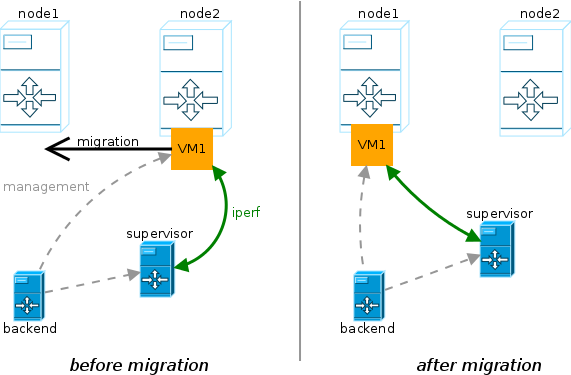
\includegraphics[width=0.9\textwidth]{methodology.png}
	\end{center}
	\caption{Methodology overview}
	\label{img:methodology}
\end{figure}


